% Отчёт по УИР 1 «Статистический анализ результатов измерений».
% Собирается и pdfLaTeX (по умолчанию в Overleaf), и XeLaTeX/LuaLaTeX.
% Рядом с этим файлом должны лежать: папка figures/ (5 png) и uir1_var12.py.
\documentclass[a4paper,12pt]{article}

% ===== Данные студента — ЗАПОЛНИТЕ =====
\newcommand{\Student}{Исаева Александра-Ирина Антовна}
\newcommand{\Group}{P3309}
\newcommand{\Teacher}{Авксентьева Е.\,Ю.}
% =======================================

\usepackage{iftex}
\ifPDFTeX
  \usepackage[T2A]{fontenc}
  \usepackage[utf8]{inputenc}
  \usepackage[english,russian]{babel}
  \IfFileExists{tempora.sty}{\usepackage{tempora}}{}
\else
  \usepackage{fontspec}
  \usepackage[english,russian]{babel}
  \IfFontExistsTF{Times New Roman}{\setmainfont{Times New Roman}}{%
    \IfFontExistsTF{Liberation Serif}{\setmainfont{Liberation Serif}}{\setmainfont{CMU Serif}}}
  \IfFontExistsTF{Courier New}{\setmonofont{Courier New}}{%
    \IfFontExistsTF{Liberation Mono}{\setmonofont{Liberation Mono}}{\setmonofont{CMU Typewriter Text}}}
\fi

\usepackage[left=25mm,right=15mm,top=20mm,bottom=20mm]{geometry}
\usepackage{amsmath,amssymb}
\usepackage{graphicx}
\usepackage{float}
\usepackage{array,multirow,booktabs}
\usepackage[labelsep=period]{caption}
\usepackage{indentfirst}
\usepackage{enumitem}
\usepackage{xcolor}
\usepackage{fvextra}
\usepackage[hidelinks]{hyperref}

\graphicspath{{figures/}}
\setlength{\parindent}{1.25cm}
\linespread{1.15}
\emergencystretch=3em
\setlist{nosep,leftmargin=*}
\renewcommand{\arraystretch}{1.15}
\captionsetup[table]{justification=raggedleft,singlelinecheck=off}

\fvset{breaklines=true,breakafter={,(=+},numbers=left,numbersep=4pt,fontsize=\scriptsize,frame=single,framesep=2mm,rulecolor=\color{gray!60}}

\begin{document}

% ---------------- Титульный лист ----------------
\begin{titlepage}
\centering
Министерство науки и высшего образования Российской Федерации\\
Федеральное государственное автономное образовательное учреждение высшего образования\\
\textbf{«Национальный исследовательский университет ИТМО»}\\[4pt]
Факультет программной инженерии и компьютерной техники

\vfill
{\large Дисциплина «Моделирование»}\\[14pt]
{\Large\textbf{Отчёт}}\\[6pt]
{\large по учебно-исследовательской работе №\,1 (УИР\,1)}\\[6pt]
{\large\textbf{«Обработка результатов измерений:\\ статистический анализ числовой последовательности»}}\\[14pt]
{\large Вариант 12}
\vfill

\begin{flushright}
\begin{tabular}{@{}l@{}}
Выполнила: \Student\\
Группа: \Group\\[8pt]
Преподаватель: \Teacher
\end{tabular}
\end{flushright}

\vfill
Санкт-Петербург, 2026
\end{titlepage}

\tableofcontents
\newpage

% ---------------- 1 ----------------
\section{Цель работы}
Изучение методов обработки и статистического анализа результатов измерений на примере заданной числовой последовательности путём оценки числовых моментов и выявления свойств последовательности на основе корреляционного анализа, а также аппроксимация закона распределения заданной последовательности по двум числовым моментам случайной величины.

% ---------------- 2 ----------------
\section{Задание и исходные данные}
В процессе исследований необходимо выполнить обработку заданной числовой последовательности (ЧП) для случаев, когда путём измерений получено 10, 20, 50, 100, 200 и 300 значений случайной величины:
\begin{itemize}
  \item рассчитать математическое ожидание, дисперсию, среднеквадратическое отклонение, коэффициент вариации, доверительные интервалы для математического ожидания с доверительными вероятностями 0,9; 0,95 и 0,99, а также относительные отклонения этих величин от значений, полученных для выборки из 300 величин;
  \item построить график значений ЧП и определить её характер (возрастающая/убывающая, периодичная);
  \item выполнить автокорреляционный анализ и определить, можно ли ЧП считать случайной;
  \item построить гистограмму распределения частот;
  \item аппроксимировать закон распределения по двум начальным моментам, реализовать генератор случайных величин, сгенерировать последовательность и сравнить её с заданной (числовые моменты, автокорреляция, гистограмма, коэффициент корреляции).
\end{itemize}

Исходные данные: заданная числовая последовательность из 300 значений. Первые значения последовательности: 107{,}28, 127{,}83, 408{,}35, 98{,}89, 701{,}76, \ldots{} Минимальное значение $x_{\min}=20{,}67$, максимальное $x_{\max}=1175{,}26$, медиана $235{,}10$.

% ---------------- 3 ----------------
\section{Методика расчёта}
\subsection{Числовые моменты}
По выборке $X_1,\dots,X_n$ рассчитываются состоятельные несмещённые оценки:
\begin{gather}
\tilde m=\frac{1}{n}\sum_{i=1}^{n}X_i,\qquad
\tilde D=\frac{1}{n-1}\sum_{i=1}^{n}\left(X_i-\tilde m\right)^2,\\
\tilde\sigma=\sqrt{\tilde D},\qquad \nu=\frac{\tilde\sigma}{\tilde m}.
\end{gather}

\subsection{Доверительный интервал}
Оценка $\tilde m$ при достаточно большом $n$ распределена нормально со среднеквадратическим отклонением $\sigma_{\tilde m}=\tilde\sigma/\sqrt n$. Доверительный интервал для математического ожидания с доверительной вероятностью $p$:
\begin{equation}
\left(\tilde m-\varepsilon_p;\ \tilde m+\varepsilon_p\right),\qquad
\varepsilon_p=t_p\,\frac{\tilde\sigma}{\sqrt n},\qquad t_p=\Phi^{-1}\!\left(\frac{1+p}{2}\right),
\end{equation}
где $t_{0{,}9}=1{,}645$, $t_{0{,}95}=1{,}960$, $t_{0{,}99}=2{,}576$. В таблицы заносится полуинтервал в виде $\pm\varepsilon_p$.

\subsection{Относительные отклонения}
\begin{equation}
\delta=\frac{a_n-a_{300}}{a_{300}}\cdot 100\%,
\end{equation}
где $a_n$~--- значение характеристики, рассчитанное по $n$ значениям, $a_{300}$~--- эталонное значение по 300 значениям. Для сгенерированной ЧП (форма 2) эталоном служат одноимённые значения заданной ЧП при том же $n$.

\subsection{Коэффициент автокорреляции}
Коэффициент автокорреляции со сдвигом $k$~--- коэффициент корреляции Пирсона между последовательностями $X_1,\dots,X_{n-k}$ и $X_{1+k},\dots,X_n$:
\begin{equation}
r(k)=\frac{\sum_{i=1}^{n-k}\left(X_i-\bar X'\right)\left(X_{i+k}-\bar X''\right)}
{\sqrt{\sum_{i=1}^{n-k}\left(X_i-\bar X'\right)^2\sum_{i=1}^{n-k}\left(X_{i+k}-\bar X''\right)^2}}.
\end{equation}
Для независимой последовательности $r(k)\approx 0$; значимость оценивается по границе $\pm 1{,}96/\sqrt n=\pm0{,}113$ при $n=300$.

% ---------------- 4 ----------------
\section{Результаты исследования}

\subsection{Числовые характеристики заданной ЧП}
Результаты расчёта сведены в таблицу~\ref{tab:f1} (форма 1).

\begin{table}[H]
\caption{Характеристики заданной ЧП \hfill Форма 1}\label{tab:f1}
\centering\small
\begin{tabular}{|l|c|r|r|r|r|r|r|}
\hline
\multirow{2}{*}{Характеристика} & & \multicolumn{6}{c|}{Количество случайных величин} \\ \cline{3-8}
 & & 10 & 20 & 50 & 100 & 200 & 300 \\ \hline
\multirow{2}{*}{Мат.\,ож.} & знач. & 296{,}357 & 308{,}568 & 271{,}816 & 276{,}942 & 265{,}089 & 276{,}478 \\
 & \% & 7{,}2 & 11{,}6 & \ensuremath{-}1{,}7 & 0{,}2 & \ensuremath{-}4{,}1 & --- \\ \hline
\multirow{2}{*}{Дов.\,инт.\,(0,9)} & знач. & $\pm$97{,}09 & $\pm$74{,}66 & $\pm$36{,}90 & $\pm$26{,}50 & $\pm$18{,}34 & $\pm$16{,}25 \\
 & \% & 497{,}3 & 359{,}3 & 127{,}0 & 63{,}0 & 12{,}8 & --- \\ \hline
\multirow{2}{*}{Дов.\,инт.\,(0,95)} & знач. & $\pm$115{,}69 & $\pm$88{,}97 & $\pm$43{,}97 & $\pm$31{,}58 & $\pm$21{,}86 & $\pm$19{,}37 \\
 & \% & 497{,}3 & 359{,}3 & 127{,}0 & 63{,}0 & 12{,}8 & --- \\ \hline
\multirow{2}{*}{Дов.\,инт.\,(0,99)} & знач. & $\pm$152{,}05 & $\pm$116{,}92 & $\pm$57{,}79 & $\pm$41{,}50 & $\pm$28{,}73 & $\pm$25{,}46 \\
 & \% & 497{,}3 & 359{,}3 & 127{,}0 & 63{,}0 & 12{,}8 & --- \\ \hline
\multirow{2}{*}{Дисперсия} & знач. & 34842{,}7 & 41209{,}8 & 25163{,}7 & 25957{,}9 & 24872{,}9 & 29298{,}2 \\
 & \% & 18{,}9 & 40{,}7 & \ensuremath{-}14{,}1 & \ensuremath{-}11{,}4 & \ensuremath{-}15{,}1 & --- \\ \hline
\multirow{2}{*}{С.\,к.\,о.} & знач. & 186{,}66 & 203{,}00 & 158{,}63 & 161{,}11 & 157{,}71 & 171{,}17 \\
 & \% & 9{,}1 & 18{,}6 & \ensuremath{-}7{,}3 & \ensuremath{-}5{,}9 & \ensuremath{-}7{,}9 & --- \\ \hline
\multirow{2}{*}{К-т вариации} & знач. & 0{,}630 & 0{,}658 & 0{,}584 & 0{,}582 & 0{,}595 & 0{,}619 \\
 & \% & 1{,}7 & 6{,}3 & \ensuremath{-}5{,}7 & \ensuremath{-}6{,}0 & \ensuremath{-}3{,}9 & --- \\ \hline
\end{tabular}

\smallskip
\footnotesize \%~--- относительные отклонения рассчитанных значений от значений, полученных для выборки из трёхсот величин.
\end{table}

Пример расчёта для $n=300$: $\sigma_{\tilde m}=171{,}167/\sqrt{300}=9{,}882$, $\varepsilon_{0{,}95}=1{,}960\cdot9{,}882=19{,}37$. Таким образом, с доверительной вероятностью 0,9; 0,95 и 0,99 математическое ожидание находится соответственно в интервалах $(260{,}2;\,292{,}7)$, $(257{,}1;\,295{,}8)$ и $(251{,}0;\,301{,}9)$.

\textbf{Выводы.}
\begin{enumerate}
  \item При малом объёме выборки (10--20 значений) оценки ненадёжны: математическое ожидание отклоняется от эталонного на 7{,}2\% и 11{,}6\%, дисперсия~--- до 40{,}7\%, а полуширина доверительного интервала в 6{,}0 и 4{,}6 раза больше, чем при $n=300$.
  \item Начиная с $n\approx 50$--$100$ оценки математического ожидания и коэффициента вариации стабилизируются (отклонения не превышают 4\% и 6\% соответственно).
  \item Дисперсия сходится медленнее остальных моментов (отклонение \ensuremath{-}15{,}1\% даже при $n=200$), так как является моментом второго порядка и чувствительна к редким большим значениям.
  \item Полуинтервал уменьшается пропорционально $1/\sqrt n$ и растёт с увеличением доверительной вероятности; относительные отклонения полуинтервалов одинаковы для всех $p$, поскольку $t_p$ входит в числитель и знаменатель как общий множитель.
  \item Коэффициент вариации $\nu=0{,}6191<1$ указывает, что распределение менее «разбросано», чем экспоненциальное.
\end{enumerate}

\subsection{График значений и характер последовательности}
\begin{figure}[H]
\centering
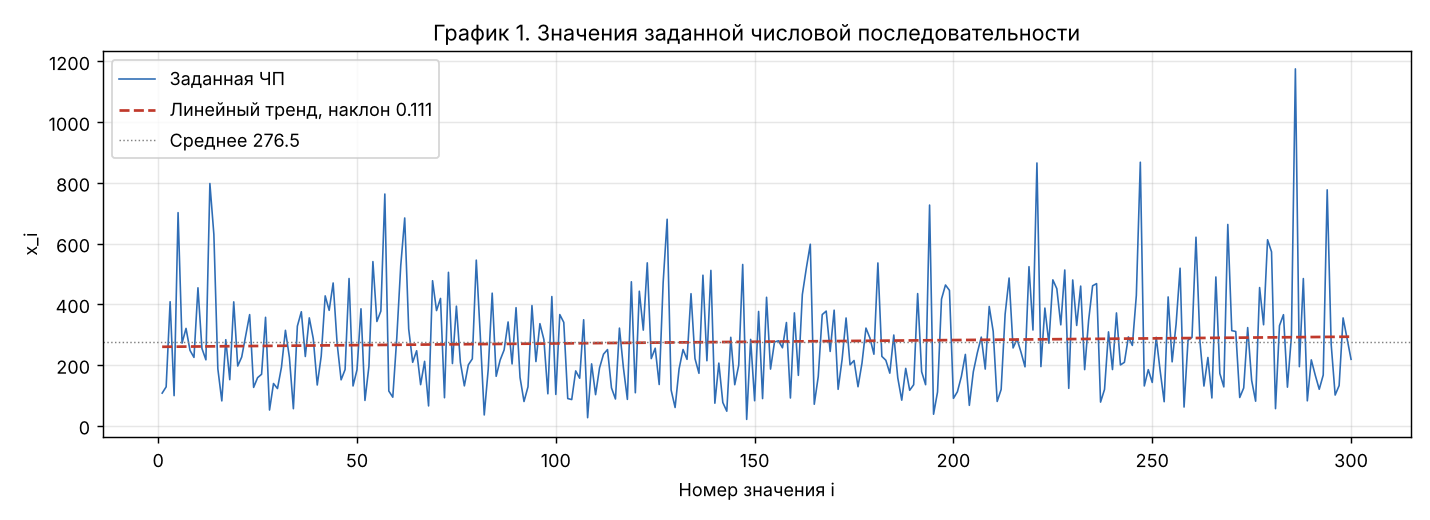
\includegraphics[width=\textwidth]{fig1_sequence.png}
\caption{График 1. Значения заданной числовой последовательности}\label{fig:seq}
\end{figure}

Для выявления тренда построена линейная регрессия $x_i=259{,}77+0{,}1110\,i$. Изменение по линии тренда на всём интервале составляет около $33{,}2$, что существенно меньше $\tilde\sigma=171{,}167$; уровень значимости наклона $p\text{-value}=0{,}33\gg0{,}05$, т.\,е. наклон статистически незначим.

\textbf{Вывод:} последовательность не является ни возрастающей, ни убывающей: значения хаотично колеблются около среднего $276{,}478$ с редкими выбросами вверх (до $1175{,}26$). Все значения положительны, распределение несимметрично (коэффициент асимметрии $1{,}31$). Периодичности визуально не наблюдается, что подтверждается автокорреляционным анализом (п.~\ref{sec:acf}).

\subsection{Автокорреляционный анализ}\label{sec:acf}
Коэффициенты автокорреляции заданной ЧП для сдвигов $k=1,\dots,10$ приведены в первой строке формы 3 (табл.~\ref{tab:f3}) и на рис.~\ref{fig:acf}.

\begin{figure}[H]
\centering
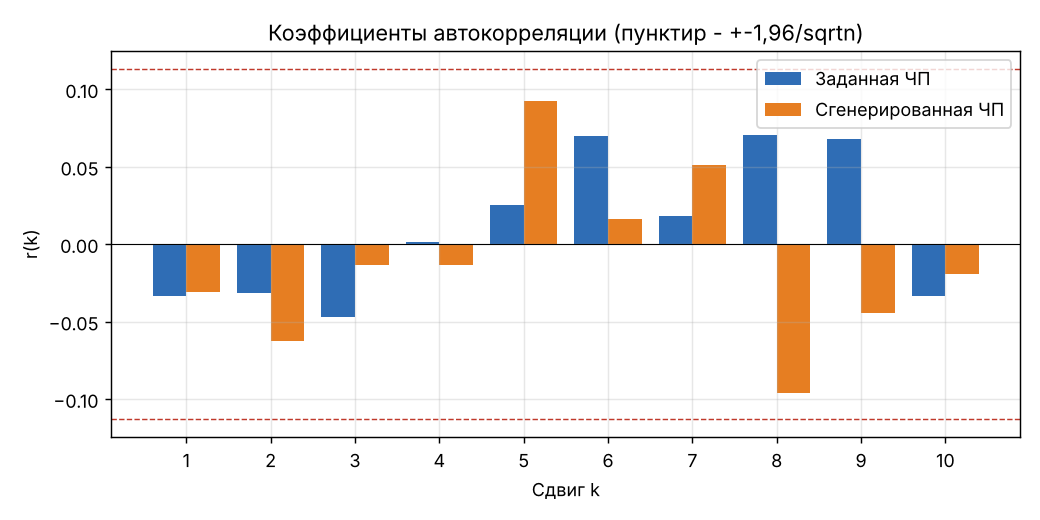
\includegraphics[width=0.82\textwidth]{fig_acf.png}
\caption{Коэффициенты автокорреляции заданной и сгенерированной ЧП}\label{fig:acf}
\end{figure}

\textbf{Вывод:} все коэффициенты автокорреляции по модулю не превышают $0{,}070$, что меньше границы значимости $0{,}113$; знаки коэффициентов меняются беспорядочно, затухающей или периодической структуры нет. Следовательно, значения последовательности можно считать некоррелированными, а саму \textbf{последовательность~--- случайной}; периодичность отсутствует.

\subsection{Гистограмма распределения частот}
Гистограмма построена с шагом 50 на интервале $[0;\,1200)$ (рис.~\ref{fig:hist}), частоты попадания приведены в табл.~\ref{tab:hist}.

\begin{figure}[H]
\centering
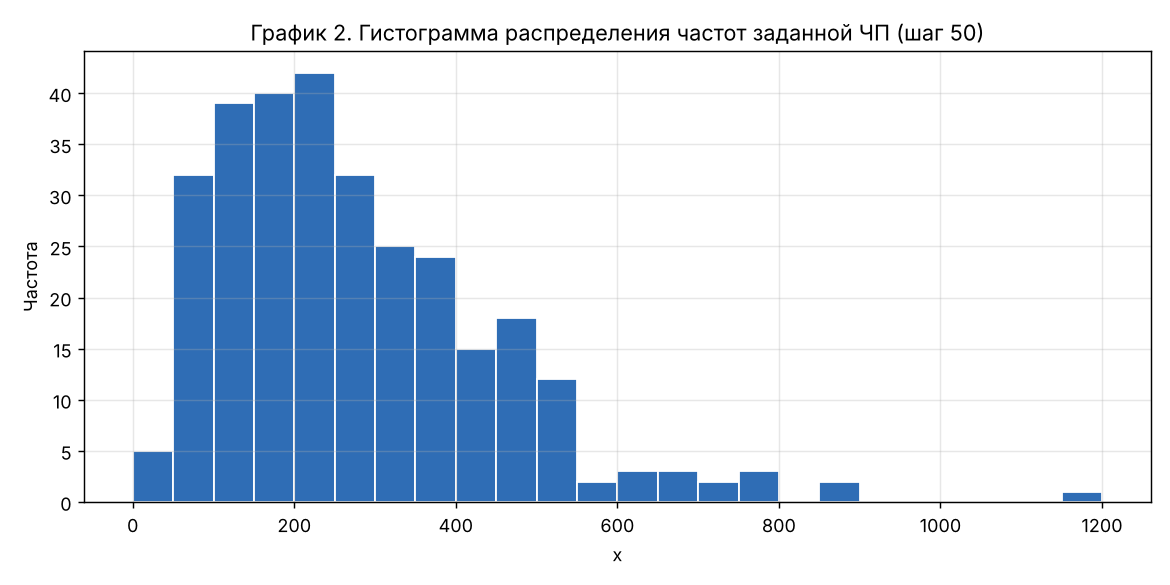
\includegraphics[width=0.85\textwidth]{fig2_histogram.png}
\caption{График 2. Гистограмма распределения частот заданной ЧП}\label{fig:hist}
\end{figure}

\begin{table}[H]
\caption{Частоты попадания значений в интервалы}\label{tab:hist}
\centering\scriptsize\setlength{\tabcolsep}{1.6pt}
\begin{tabular}{|l|*{12}{c|}}
\hline
Интервал & 0--50 & 50--100 & 100--150 & 150--200 & 200--250 & 250--300 & 300--350 & 350--400 & 400--450 & 450--500 & 500--550 & 550--600 \\ \hline
Заданная & 5 & 32 & 39 & 40 & 42 & 32 & 25 & 24 & 15 & 18 & 12 & 2 \\ \hline
Сгенерир. & 6 & 30 & 40 & 35 & 39 & 31 & 25 & 23 & 25 & 9 & 8 & 7 \\ \hline
\multicolumn{13}{c}{} \\[-6pt] \hline
Интервал & 600--650 & 650--700 & 700--750 & 750--800 & 800--850 & 850--900 & 900--950 & 950--1000 & 1000--1050 & 1050--1100 & 1100--1150 & 1150--1200 \\ \hline
Заданная & 3 & 3 & 2 & 3 & 0 & 2 & 0 & 0 & 0 & 0 & 0 & 1 \\ \hline
Сгенерир. & 8 & 3 & 4 & 2 & 3 & 0 & 0 & 2 & 0 & 0 & 0 & 0 \\ \hline
\end{tabular}
\end{table}

\textbf{Вывод:} распределение одномодальное, мода находится в области 150--250; слева~--- быстрый рост плотности от нуля, справа~--- длинный «хвост». Такая форма характерна для распределения Эрланга или гипоэкспоненциального распределения и не соответствует экспоненциальному (максимум которого находится в нуле) и равномерному.

\subsection{Аппроксимация закона распределения}
Вид аппроксимирующего закона выбирается по коэффициенту вариации $\nu=0{,}6191$:
\begin{itemize}
  \item $\nu=1$~--- экспоненциальный, $\nu>1$~--- гиперэкспоненциальный: не подходят;
  \item равномерный закон имеет $\nu\le 1/\sqrt3\approx0{,}577$ и ограниченную область значений, что противоречит гистограмме с длинным «хвостом»;
  \item $0<\nu<1$~--- нормированное распределение Эрланга $k$-го порядка ($\nu=1/\sqrt k$) или гипоэкспоненциальное.
\end{itemize}

Поскольку $1/\nu^2=2{,}609$ не является целым числом, распределение Эрланга точно не воспроизводит $\nu$ (при $k=3$: $\nu=0{,}577$; при $k=2$: $\nu=0{,}707$), а двухфазное гипоэкспоненциальное распределение реализует только $\nu\in[1/\sqrt2;\,1)$. Поэтому выбрано \textbf{трёхфазное гипоэкспоненциальное распределение}~--- сумма трёх независимых экспоненциально распределённых величин со средними $t_1$ и $t_2=t_3$, которое реализует $\nu\in[1/\sqrt3;\,1)$.

Параметры определяются из равенства двух первых моментов:
\begin{equation}
\begin{cases}
t_1+2t_2=\tilde m,\\
t_1^2+2t_2^2=\nu^2\tilde m^2,
\end{cases}
\quad\Rightarrow\quad
t_2=\frac{\tilde m\left(2-\sqrt{6\nu^2-2}\right)}{6},\qquad t_1=\tilde m-2t_2 .
\end{equation}

При $\tilde m=276{,}478$, $\nu=0{,}6191$: $\sqrt{6\nu^2-2}=0{,}5474$, откуда
\[
t_1=142{,}611\ (\lambda_1=1/t_1=0{,}00701),\qquad t_2=t_3=66{,}933\ (\lambda_2=\lambda_3=0{,}01494).
\]
Проверка: $t_1+2t_2=276{,}478$, $\sqrt{t_1^2+2t_2^2}\,/\,(t_1+2t_2)=0{,}6191$~--- оба момента воспроизводятся точно.

Плотность распределения (свёртка экспоненциального распределения с параметром $\lambda_1$ и распределения Эрланга 2-го порядка с параметром $\lambda_2$):
\begin{equation}
f(t)=\frac{\lambda_1\lambda_2^2}{(\lambda_2-\lambda_1)^2}\left[e^{-\lambda_1 t}-e^{-\lambda_2 t}\bigl(1+(\lambda_2-\lambda_1)\,t\bigr)\right],\quad t\ge0 .
\end{equation}

Для сравнения рассмотрено нормированное распределение Эрланга 3-го порядка с параметром $\lambda=3/\tilde m=0{,}01085$.

Согласие с данными проверено критерием Колмогорова--Смирнова (критическое значение при $\alpha=0{,}05$: $1{,}36/\sqrt{300}=0{,}079$):
\begin{table}[H]
\caption{Проверка согласия по критерию Колмогорова--Смирнова}
\centering
\begin{tabular}{|l|c|c|c|}
\hline
Закон распределения & $\nu$ & Статистика $D$ & $p$-value \\ \hline
Гипоэкспоненциальный (3 фазы) & 0{,}6191 & 0{,}0429 & 0{,}624 \\ \hline
Эрланга 3-го порядка & 0{,}5774 & 0{,}0594 & 0{,}232 \\ \hline
Экспоненциальный & 1 & 0{,}1952 & $<0{,}0001$ \\ \hline
\end{tabular}
\end{table}

\textbf{Вывод:} гипоэкспоненциальный закон согласуется с данными лучше остальных ($D=0{,}0429<0{,}079$, гипотеза не отвергается), экспоненциальный закон отвергается.

\subsection{Алгоритм генератора случайных величин}
Генерация выполняется методом обратной функции: экспоненциально распределённая величина со средним $t$ получается из равномерно распределённой на $(0;1)$ величины $r$ как $-t\ln r$. Гипоэкспоненциальная величина~--- сумма трёх таких величин:
\begin{equation}
\tau=-t_1\ln r_1-t_2\ln r_2-t_2\ln r_3 = -142{,}611\ln r_1-66{,}933\ln r_2-66{,}933\ln r_3,
\end{equation}
где $r_1,r_2,r_3$~--- независимые псевдослучайные числа, равномерно распределённые на $(0;1)$.

Алгоритм программы (приложение~\ref{app:code}):
\begin{enumerate}
  \item считать 300 значений заданной последовательности из файла;
  \item для $n=10,20,50,100,200,300$ вычислить $\tilde m,\tilde D,\tilde\sigma,\nu,\varepsilon_p$ и относительные отклонения (форма 1);
  \item вычислить коэффициенты автокорреляции $r(1),\dots,r(10)$ и линейный тренд;
  \item по $\tilde m$ и $\nu$ рассчитать параметры $t_1,t_2$ аппроксимирующего закона;
  \item сгенерировать 300 значений $\tau$ по формуле выше (для воспроизводимости зафиксировано начальное значение генератора);
  \item рассчитать характеристики сгенерированной ЧП (форма 2), её автокорреляцию (форма 3), коэффициент корреляции с заданной ЧП;
  \item построить графики.
\end{enumerate}
\subsection{Сравнение сгенерированной и заданной последовательностей}

\paragraph{а) Плотность распределения и гистограммы.}
\begin{figure}[H]
\centering
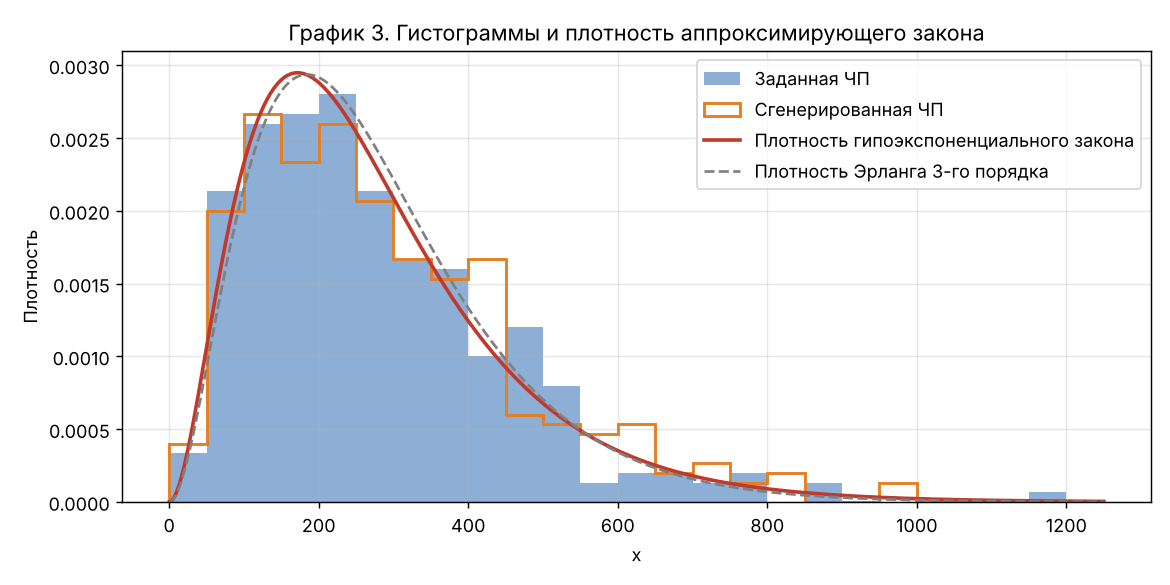
\includegraphics[width=0.9\textwidth]{fig3_approximation.png}
\caption{График 3. Гистограммы заданной и сгенерированной ЧП и плотность аппроксимирующего закона}\label{fig:approx}
\end{figure}
Плотность гипоэкспоненциального закона хорошо повторяет форму гистограммы заданной ЧП: совпадают положение моды (около 170--200), крутизна левой ветви и «хвост». Гистограмма сгенерированной ЧП располагается в той же области. Двухвыборочный критерий Колмогорова--Смирнова: $D=0{,}0500$, $p\text{-value}=0{,}848$~--- выборки статистически неразличимы.

\paragraph{б) Числовые характеристики сгенерированной ЧП.}
\begin{table}[H]
\caption{Характеристики сгенерированной случайной ЧП \hfill Форма 2}\label{tab:f2}
\centering\small
\textit{Закон распределения: гипоэкспоненциальный, $t_1=142{,}611$, $t_2=t_3=66{,}933$}\\[4pt]
\begin{tabular}{|l|c|r|r|r|r|r|r|}
\hline
\multirow{2}{*}{Характеристика} & & \multicolumn{6}{c|}{Количество случайных величин} \\ \cline{3-8}
 & & 10 & 20 & 50 & 100 & 200 & 300 \\ \hline
\multirow{2}{*}{Мат.\,ож.} & знач. & 298{,}623 & 271{,}385 & 292{,}971 & 284{,}753 & 287{,}202 & 288{,}083 \\
 & \% & 0{,}8 & \ensuremath{-}12{,}1 & 7{,}8 & 2{,}8 & 8{,}3 & 4{,}2 \\ \hline
\multirow{2}{*}{Дов.\,инт.\,(0,9)} & знач. & $\pm$77{,}38 & $\pm$61{,}39 & $\pm$41{,}55 & $\pm$29{,}67 & $\pm$21{,}35 & $\pm$17{,}14 \\
 & \% & \ensuremath{-}20{,}3 & \ensuremath{-}17{,}8 & 12{,}6 & 12{,}0 & 16{,}4 & 5{,}4 \\ \hline
\multirow{2}{*}{Дов.\,инт.\,(0,95)} & знач. & $\pm$92{,}20 & $\pm$73{,}15 & $\pm$49{,}51 & $\pm$35{,}36 & $\pm$25{,}45 & $\pm$20{,}42 \\
 & \% & \ensuremath{-}20{,}3 & \ensuremath{-}17{,}8 & 12{,}6 & 12{,}0 & 16{,}4 & 5{,}4 \\ \hline
\multirow{2}{*}{Дов.\,инт.\,(0,99)} & знач. & $\pm$121{,}17 & $\pm$96{,}14 & $\pm$65{,}06 & $\pm$46{,}47 & $\pm$33{,}44 & $\pm$26{,}84 \\
 & \% & \ensuremath{-}20{,}3 & \ensuremath{-}17{,}8 & 12{,}6 & 12{,}0 & 16{,}4 & 5{,}4 \\ \hline
\multirow{2}{*}{Дисперсия} & знач. & 22128{,}7 & 27860{,}9 & 31901{,}9 & 32541{,}4 & 33710{,}4 & 32564{,}7 \\
 & \% & \ensuremath{-}36{,}5 & \ensuremath{-}32{,}4 & 26{,}8 & 25{,}4 & 35{,}5 & 11{,}1 \\ \hline
\multirow{2}{*}{С.\,к.\,о.} & знач. & 148{,}76 & 166{,}92 & 178{,}61 & 180{,}39 & 183{,}60 & 180{,}46 \\
 & \% & \ensuremath{-}20{,}3 & \ensuremath{-}17{,}8 & 12{,}6 & 12{,}0 & 16{,}4 & 5{,}4 \\ \hline
\multirow{2}{*}{К-т вариации} & знач. & 0{,}498 & 0{,}615 & 0{,}610 & 0{,}634 & 0{,}639 & 0{,}626 \\
 & \% & \ensuremath{-}20{,}9 & \ensuremath{-}6{,}5 & 4{,}5 & 8{,}9 & 7{,}5 & 1{,}2 \\ \hline
\end{tabular}

\smallskip
\footnotesize \%~--- относительные отклонения характеристик сгенерированной случайной последовательности от одноимённых значений заданной числовой последовательности.
\end{table}

\begin{table}[H]
\caption{Коэффициенты автокорреляции \hfill Форма 3}\label{tab:f3}
\centering\footnotesize\setlength{\tabcolsep}{3pt}
\begin{tabular}{|l|*{10}{r|}}
\hline
Сдвиг ЧП & 1 & 2 & 3 & 4 & 5 & 6 & 7 & 8 & 9 & 10 \\ \hline
АК заданной ЧП & \ensuremath{-}0{,}033 & \ensuremath{-}0{,}031 & \ensuremath{-}0{,}047 & 0{,}001 & 0{,}026 & 0{,}070 & 0{,}018 & 0{,}070 & 0{,}068 & \ensuremath{-}0{,}034 \\ \hline
АК сгенерир. ЧП & \ensuremath{-}0{,}031 & \ensuremath{-}0{,}062 & \ensuremath{-}0{,}013 & \ensuremath{-}0{,}014 & 0{,}092 & 0{,}016 & 0{,}051 & \ensuremath{-}0{,}096 & \ensuremath{-}0{,}044 & \ensuremath{-}0{,}019 \\ \hline
$|\Delta r|$ & 0{,}003 & 0{,}031 & 0{,}033 & 0{,}015 & 0{,}067 & 0{,}054 & 0{,}033 & 0{,}166 & 0{,}112 & 0{,}014 \\ \hline
\% & 8 & \ensuremath{-}99 & 71 & \ensuremath{-}1054 & 261 & \ensuremath{-}77 & 186 & \ensuremath{-}237 & \ensuremath{-}165 & 42 \\ \hline
\end{tabular}
\end{table}

\begin{figure}[H]
\centering
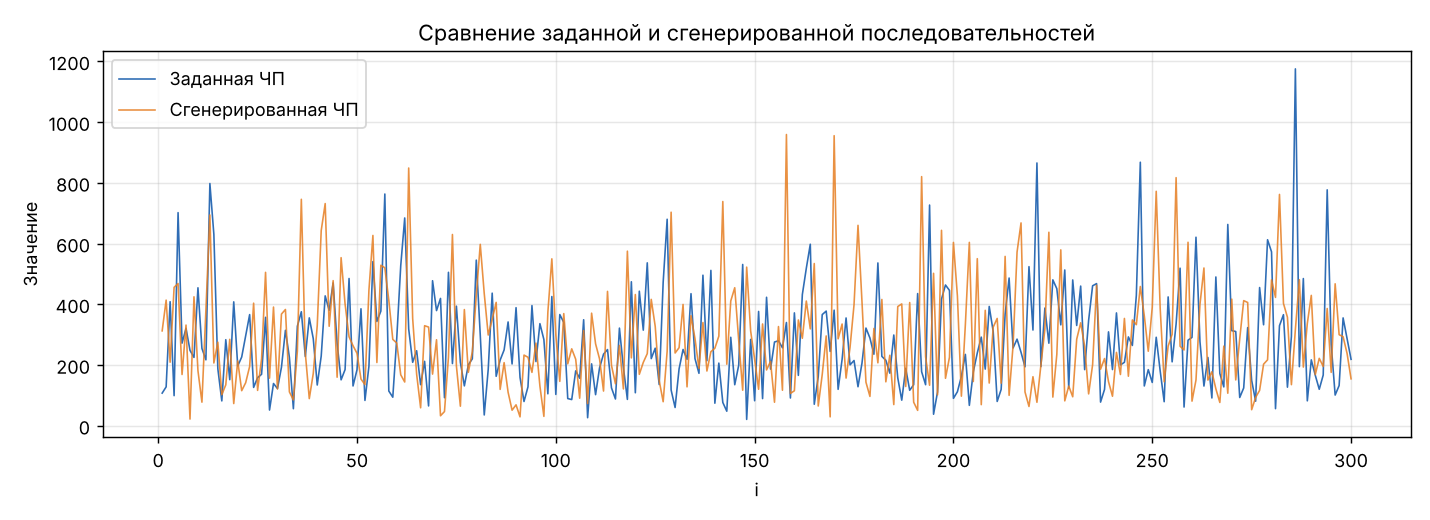
\includegraphics[width=\textwidth]{fig_compare.png}
\caption{Значения заданной и сгенерированной последовательностей}\label{fig:cmp}
\end{figure}

При $n=300$ математическое ожидание сгенерированной ЧП ($288{,}083$) отличается от заданного на 4{,}2\%, среднеквадратическое отклонение~--- на 5{,}4\%, дисперсия~--- на 11{,}1\%, коэффициент вариации ($0{,}6264$)~--- на 1{,}2\%. Эти расхождения соответствуют статистическому разбросу оценок по 300 значениям (сама заданная ЧП при разных $n$ даёт отклонения дисперсии до 15\%). При малых $n$ расхождения велики и разнонаправлены, так как обе выборки случайны.

Коэффициенты автокорреляции сгенерированной ЧП по модулю не превышают $0{,}096$ и, как и для заданной ЧП, лежат внутри границ $\pm0{,}113$, т.\,е. сгенерированная последовательность также случайна. Поскольку коэффициенты автокорреляции близки к нулю, их относительные отклонения в процентах велики и малоинформативны; показательнее абсолютная разность $|\Delta r|$, которая не превышает 0,17.

\paragraph{в) Корреляционный анализ.}
Коэффициент корреляции между заданной и сгенерированной последовательностями $r_{xy}=\ensuremath{-}0{,}0121$, что по модулю много меньше границы значимости $0{,}113$: последовательности \textbf{некоррелированы}. Это ожидаемо: генератор воспроизводит закон распределения, а не конкретные значения последовательности.

% ---------------- 5 ----------------
\section{Заключение}
\begin{enumerate}
  \item Для заданной ЧП по 300 значениям получены оценки: $\tilde m=276{,}478$, $\tilde D=29298{,}2$, $\tilde\sigma=171{,}167$, $\nu=0{,}6191$; доверительный интервал для математического ожидания с вероятностью 0,95~--- $276{,}478\pm19{,}37$. Оценки, полученные по 10--20 значениям, отличаются от эталонных на десятки процентов; приемлемая точность достигается при $n\ge100$.
  \item Последовательность не имеет тренда (наклон незначим) и периодичности.
  \item Все коэффициенты автокорреляции незначимы ($|r(k)|\le0{,}070<0{,}113$), поэтому последовательность можно считать случайной.
  \item Гистограмма одномодальная, скошенная вправо; с учётом $\nu=0{,}6191$ для описания ЧП предложен трёхфазный гипоэкспоненциальный закон с параметрами $t_1=142{,}611$, $t_2=t_3=66{,}933$, который точно воспроизводит два первых момента и лучше распределения Эрланга 3-го порядка согласуется с данными по критерию Колмогорова--Смирнова ($p=0{,}624$).
  \item Сгенерированная по этому закону последовательность близка к заданной по числовым моментам (расхождения около 1--11\% при $n=300$), форме гистограммы и автокорреляционным свойствам, при этом не коррелирует с заданной ($r_{xy}=\ensuremath{-}0{,}0121$). Качество аппроксимации можно считать хорошим.
\end{enumerate}

\appendix
\section{Программа расчёта и генератора}\label{app:code}
\VerbatimInput{uir1_var12.py}

\end{document}
